\newpage
\section{Detection and Segmentation}

\subsection{Semantic Segmentation}
Label each pixel in the image with a category label. 对多个重叠物体不作区分.

Semantic Segmentation Idea:

\subsubsection{Sliding Window}
非常低效. 对重叠部分没利用共享的特征. 
\begin{figure}[!htb]
    \centering
    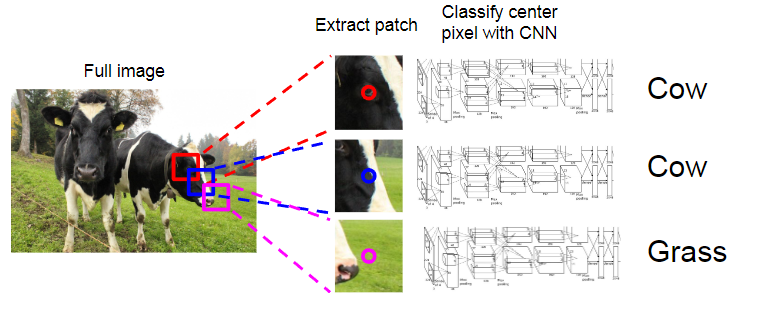
\includegraphics[width=0.42\textwidth]{pic/Lec11/sliding window.png}
    \caption{Sliding Window}
\end{figure}
\subsubsection{Fully Convolutional}
源分辨率的卷积非常昂贵. 训练数据非常贵. 
\begin{figure}[!htb]
    \centering
    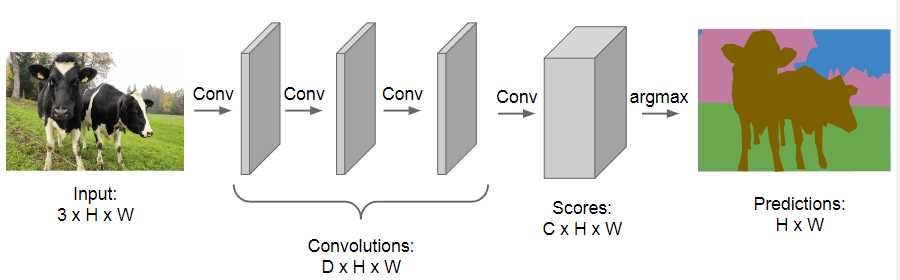
\includegraphics[width=0.42\textwidth]{pic/Lec11/Fully Convolutional.png}
    \caption{Fully Convolutional}
\end{figure}
    
改进: with downsampling and upsampling inside
\begin{figure}[!htb]
    \centering
    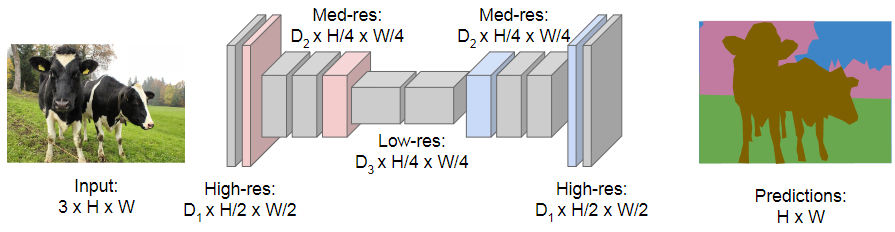
\includegraphics[width=0.309\textwidth]{pic/Lec11/downsampling and upsampling.png}
    \caption{downsampling and upsampling}
\end{figure}
    
\begin{itemize}
    \item Downsampling: Pooling, strided, convolution
    \item Upsampling: Unpooling or strided transpose convolution
\end{itemize}

\begin{figure}[!htb]
    \centering
    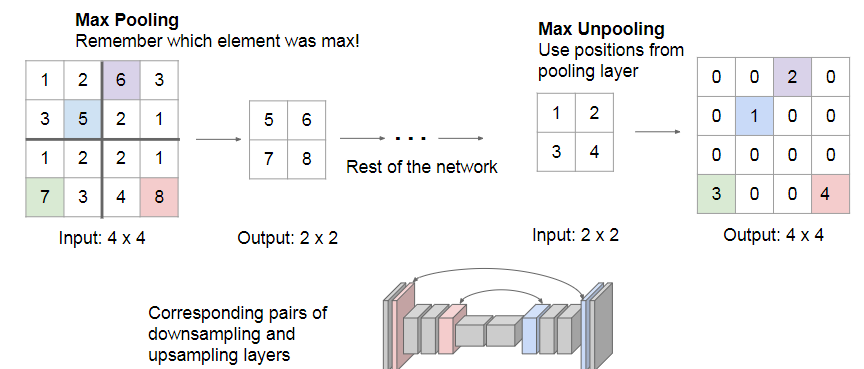
\includegraphics[width=0.42\textwidth]{pic/lec11/Max Unpooling.png}
    \caption{Max Unpooling: 空值可以更好的传递pooling 丢失的信息.}
\end{figure}

\begin{figure}[!htb]
    \centering
    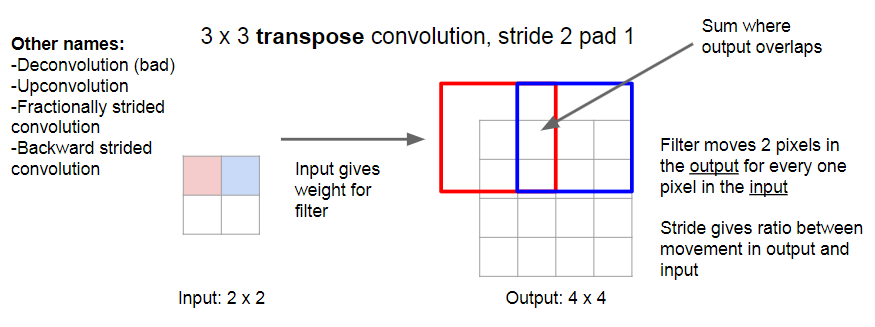
\includegraphics[width=0.42\textwidth]{pic/lec11/Transpose Convolution}
    \caption{Learnable Upsampling: Transpose Convolution(如果用矩乘表示卷积, 那么此方法是卷积的转置)}
\end{figure}

\subsection{Classification + Localization}
两个loss通过超参数加权得到最终loss, 用此反向传播. 

\begin{figure}[!htb]
    \centering
    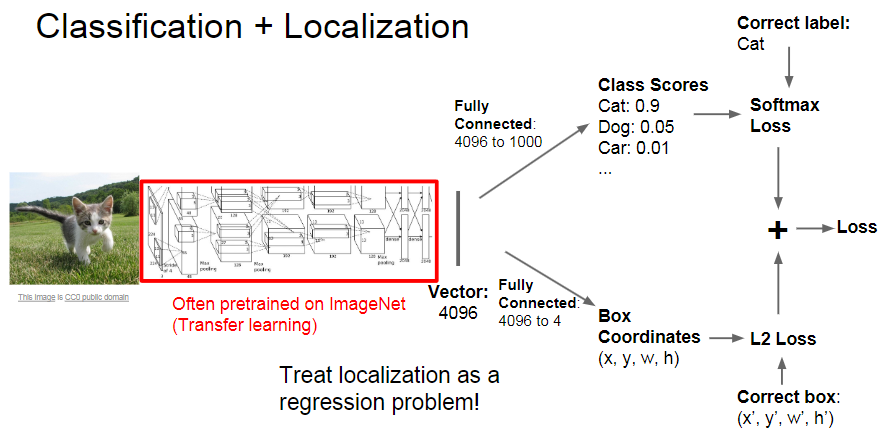
\includegraphics[width=0.42\textwidth]{pic/lec11/Classification + Localization}
    \caption{Classification + Localization}
\end{figure}
\begin{figure}[!htb]
    \centering
    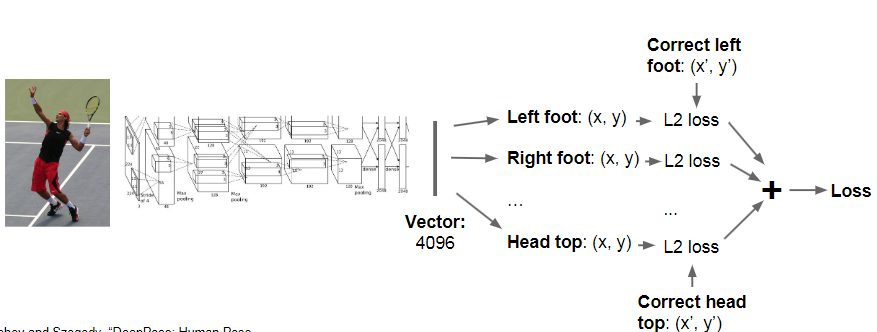
\includegraphics[width=0.42\textwidth]{pic/lec11/Aside Human Pose Estimation}
    \caption{Aside: Human Pose Estimation}
\end{figure}

\subsection{Object Detection}
As Regression: Each image needs a different number of outputs. 

As Classification: Sliding Window. 获取许多 crop, 对其每个跑CNN. 
Problem: Need to apply CNN to huge number of locations and scales, very computationally expensive!

\subsubsection{Region Proposals}
\begin{itemize}
    \item Find ``blobby'' image regions that are likely to contain objects
    \item Relatively fast to run. 
\end{itemize}
准确率不高, 但召回率高. 

\subsubsection{R-CNN}
\begin{figure}[!htb]
    \centering
    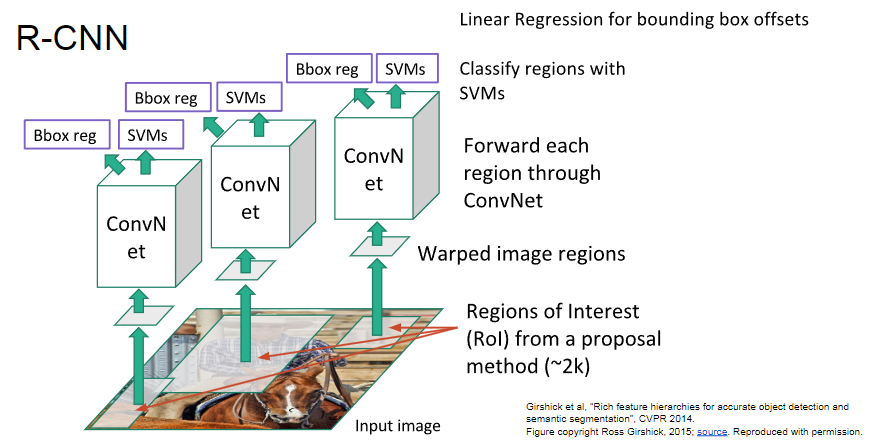
\includegraphics[width=0.42\textwidth]{pic/lec11/R-CNN}
    \caption{R-CNN}
\end{figure}

Problems: 
\begin{itemize}
    \item 还是很贵
    \item 训练慢
    \item 测试也慢
\end{itemize}

\subsubsection{Fast R-CNN}
\begin{figure}[!htb]
    \centering
    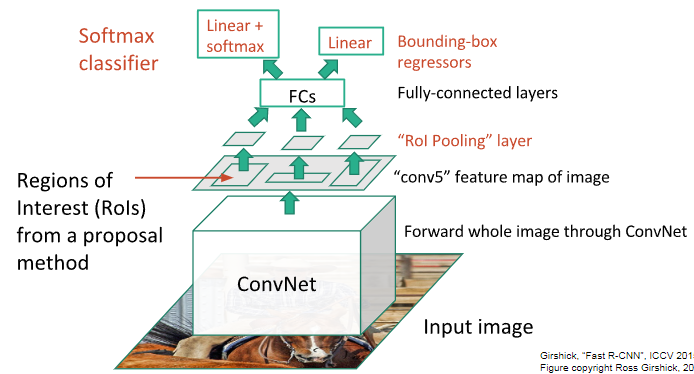
\includegraphics[width=0.309\textwidth]{pic/Lec11/Fast R-CNN}
    \caption{Fast R-CNN}
\end{figure}

\subsubsection{Faster R-CNN}
Make CNN do proposals!
\begin{figure}[!htb]
    \centering
    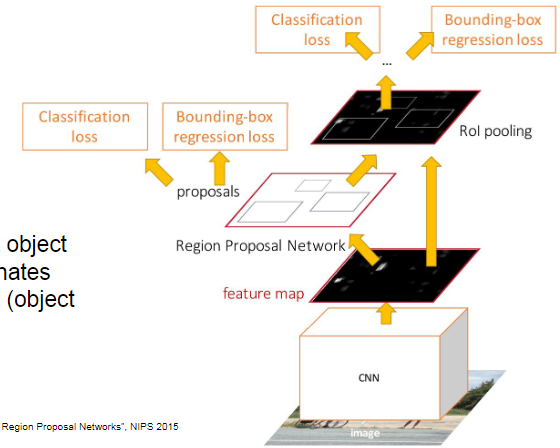
\includegraphics[width=0.309\textwidth]{pic/Lec11/Faster R-CNN}
    \caption{Faster R-CNN}
\end{figure}

Jointly train with 4 losses:
\begin{enumerate}
    \item RPN classify object / not object
    \item RPN regress box coordinates
    \item Final classification score (objec classes)
    \item Final box coordinates
\end{enumerate}
做了实验后表明只需要学一个. 

\subsubsection{Detection without Proposals: YOLO / SSD}
\begin{figure}[!htb]
    \centering
    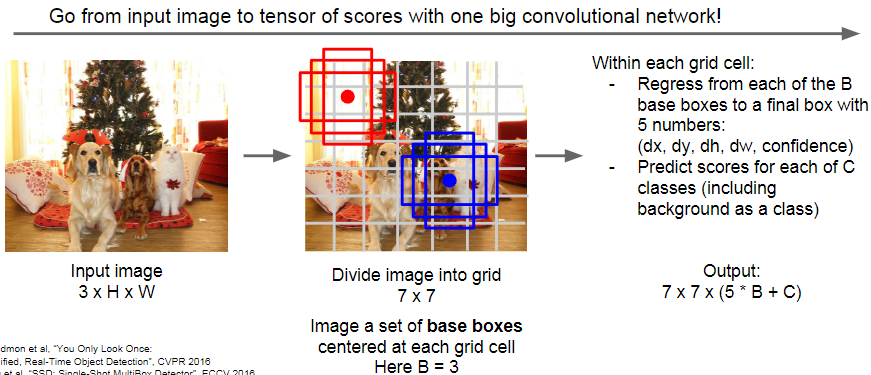
\includegraphics[width=0.42\textwidth]{pic/Lec11/Detection without Proposals}
    \caption{Detection without Proposals}
\end{figure}

\begin{figure}[!htb]
    \centering
    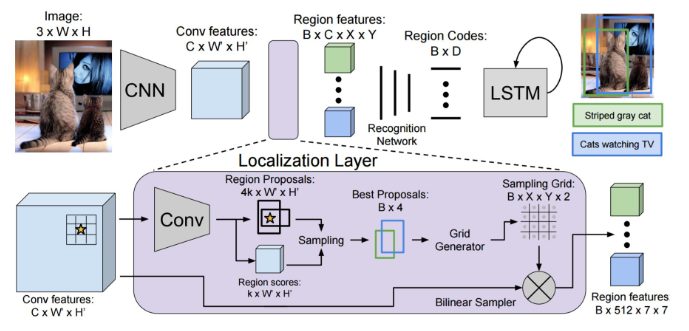
\includegraphics[width=0.42\textwidth]{pic/Lec11/Object Detection + Captioning = Dense Captioning}
    \caption{Aside: Object Detection + Captioning = Dense Captioning}
\end{figure}

\subsection{Instance Segmentation}

\subsubsection{Mask R-CNN}
\begin{figure}[!htb]
    \centering
    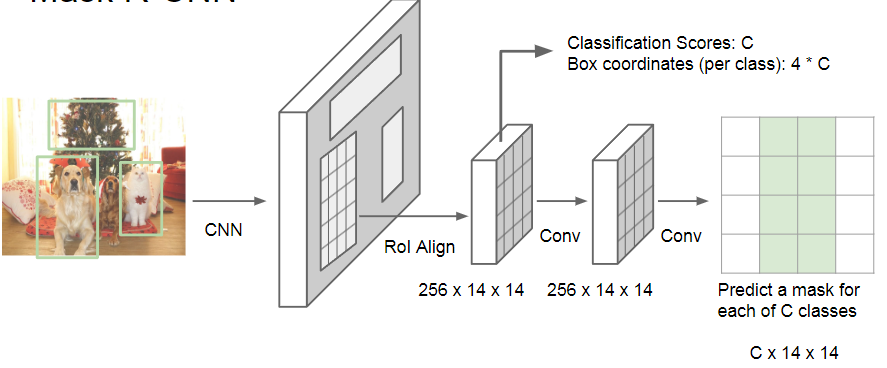
\includegraphics[width=0.42\textwidth]{pic/Lec11/Mask R-CNN}
    \caption{Mask R-CNN}
\end{figure}

Also does pose